%%%%%%%%%%%%%%%%%%%%%%
\documentclass{doublecol-new}
%%%%%%%%%%%%%%%%%%%%%%

\usepackage{natbib,stfloats}
\usepackage{mathrsfs}
\usepackage{graphicx}

\def\newblock{\hskip .11em plus .33em minus .07em}

\theoremstyle{TH}{
\newtheorem{lemma}{Lemma}
\newtheorem{theorem}[lemma]{Theorem}
\newtheorem{corrolary}[lemma]{Corrolary}
\newtheorem{conjecture}[lemma]{Conjecture}
\newtheorem{proposition}[lemma]{Proposition}
\newtheorem{claim}[lemma]{Claim}
\newtheorem{stheorem}[lemma]{Wrong Theorem}
\newtheorem{algorithm}{Algorithm}
}

\theoremstyle{THrm}{
\newtheorem{definition}{Definition}[section]
\newtheorem{question}{Question}[section]
\newtheorem{remark}{Remark}
\newtheorem{scheme}{Scheme}
}

\theoremstyle{THhit}{
\newtheorem{case}{Case}[section]
}

\makeatletter
\def\theequation{\arabic{equation}}

%\JOURNALNAME{\TEN{\it Int. J. System Control and Information
%Processing,
%Vol. \theVOL, No. \theISSUE, \thePUBYEAR\hfill\thepage}}%
%
%\def\BottomCatch{%
%\vskip -10pt
%\thispagestyle{empty}%
%\begin{table}[b]%
%\NINE\begin{tabular*}{\textwidth}{@{\extracolsep{\fill}}lcr@{}}%
%\\[-12pt]
%Copyright \copyright\ 2012 Inderscience Enterprises Ltd. & &%
%\end{tabular*}%
%\vskip -30pt%
%%%\vskip -35pt%
%\end{table}%
%}
\makeatother

%%%%%%%%%%%%%%%%%
\begin{document}%
%%%%%%%%%%%%%%%%%

\setcounter{page}{1}

%\LRH{F. Wang et~al.}

\RRH{An ontology and frequency-based approach to recommend activities in scientific workflows}

%\VOL{x}
%
%\ISSUE{x}
%
%\PUBYEAR{xxxx}

\BottomCatch

%\CLline

%\PUBYEAR{201X}

\subtitle{}

\title{An ontology and frequency-based approach to recommend activities in scientific workflows}

%
%\authorA{Fusheng Wang}
%%
%\affA{Department of Biomedical Informatics,\\ Emory University,\\ Atlanta, GA, USA \\
%Fax: +1 \qquad E-mail: fusheng.wang@emory.edu}
%%
%%
%\authorB{Fusheng Wang}
%\affB{Department of Biomedical Informatics,\\ Emory University,\\ Atlanta, GA, USA \\
%Fax: +1 \qquad E-mail: fusheng.wang@emory.edu}
%

%
%\authorA{Fusheng Wang\footnote{Work done while working at Siemens Corporate Research.} }
%
%\affA{Department of Biomedical Informatics, Emory University
%\newline
%36 Eagle Row, Ste 589, Atlanta, GA 30322, USA}
%
%
%
%\authorB{\footnotesize Cristobal Vergara-Niedermayr\footnote{Work done while working at Siemens Corporate Research.}}
%\affB{Oracle \newline
 %New Jersey, USA}
%
%
%\authorC{Peiya Liu}
%\affC{Department of Integrated Data Systems, Siemens Corporate
%Research \newline 755 College Road East, Princeton 08540, USA}

\begin{abstract}
The number of activities provided by scientific workflow management systems is large,
which requires scientists to know many of them to take advantage of the reusability
of these systems. To minimize this problem, the literature presents some techniques to recommend activities during the scientific workflow construction. In this paper we specified and developed a hybrid activity recommendation system considering information on frequency, input and outputs of activities and ontological annotations. Additionally, this project presents a modelling of activities recommendation as a classification problem, tested using \(5\) classifiers; \(5\) regressors; and a composite approach which uses a SVM classifier, combining the results of other classifiers and
regressors to recommend; and Rotation Forest, an ensemble of classifiers. The proposed techniques were compared to related techniques and to classifiers and regressors, using \(10\)-fold-cross-validation, achieving a MRR at least \(70\%\) greater than those obtained by classical techniques.
\end{abstract}

\KEYWORD{Recommendation systems. Ontologies. Scientific Workflows Management Systems. Recommender Systems.}

%\REF{to this paper should be made as follows: Rodr\'{\i}guez
%Bol\'{\i}var, M.P. and Sen\'{e}s Garc\'{\i}a, B. (xxxx) `The
%corporate environmental disclosures on the internet: the case of
%IBEX 35 Spanish companies', {\it International Journal of Metadata,
%Semantics and Ontologies}, Vol. x, No. x, pp.xxx\textendash xxx.}
%
%\begin{bio}
%Manuel Pedro Rodr\'iguez Bol\'ivar received his PhD in Accounting at
%the University of Granada. He is a Lecturer at the Department of
%Accounting and Finance, University of Granada. His research
%interests include issues related to conceptual frameworks of
%accounting, diffusion of financial information on Internet, Balanced
%Scorecard applications and environmental accounting. He is author of
%a great deal of research studies published at national and
%international journals, conference proceedings as well as book
%chapters, one of which has been edited by Kluwer Academic
%Publishers.\vs{9}
%
%\noindent Bel\'en Sen\'es Garc\'ia received her PhD in Accounting at
%the University of Granada. She is a Lecturer at the Department of
%Accounting and Finance, University of Granada. Her research
%interests are related to cultural, institutional and historic
%accounting and in environmental accounting. She has published
%research papers at national and international journals, conference
%proceedings as well as chapters of books.\vs{8}
%
%\noindent Both authors have published a book about environmental
%accounting edited by the Institute of Accounting and Auditing,
%Ministry of Economic Affairs, in Spain in October 2003.
%\end{bio}


\maketitle

\section*{Introduction}
The number of research projects using intensive computing has been growing in areas such as biology, physics, and astronomy. One of the tools to assist in the management and construction of intensive computing experiments are the workflows management systems. \emph{Scientific Workflows} represent structured and ordered processes, constructed manually, semi-automatically or automatically to solve scientific problems using activities, which can be: i) source code blocks; (ii) services; or iii) finished workflows~(\cite{Wang2010}). These systems facilitate the creation of new experiments, sharing of results and reuse of existing activities.

Nowadays, there are a large number of activities available in repositories such as \cite{ROURE2015} which stores more than 2,500 workflows and \cite{BioCatalogue2015}, which provides more than 2,464 services. The large number of activities and the low reuse of some activities and workflows motivate the construction of techniques to recommend activities to the scientists during the composition of workflows (\cite{Wang2010}).

In the workflow management systems, activities are typically represented as graphical icons with drag and drop functionality. Thus, it is possible to construct computational experiments by dragging icons and filling in input parameters. Most of these systems provide sets of basic activities that can be used in different domains, for example, an activity that calculates the average value of a dataset is applicable in biology, physics, astronomy, and other areas. However, there is a precondition for reusing and/or creating workflows: knowing the available activities.

In order to minimize the problem of knowing a large number of activities, several techniques were proposed to recommend activities or to compose workflows. In the first case, which aims to serve an expert user in these systems, during the construction of the workflow, activities are recommended to help to complete the workflow. In the second case, whose goal is to serve a less expert user, several workflows are built and the user should select which one most satisfies him/her need.

This paper presents a hybrid approach for recommending activities in scientific workflows based on the frequency of activities combined with the use of semantics, considering datasets with no provenance information, and without reliability information about the authors of the services and workflows. We also propose a modeling of the problem of recommending activities in scientific workflows to be used by classifiers such as: Support Vector Machine (SVM), Naive Bayes (NB), K-Nearest-Neighbor (KNN), Classification and Regression Trees, and Neural Network (MLP). The following regressors were also used: Support Vector Regression (SVR), CART, Neural Network, Multivariate Adaptive Regression Splines (MARS) and Binomial Regression (RB). At last, a comparison of our approach and the approaches from the related literature is presented.

Section \emph{Relate Work} describes the techniques proposed in the related literature are described. Section \emph{Materials and Methods} presents the data source, selected sample, and  the modelling of the problem as a artificial intelligence classification problem.
Section \emph{Proposed Solutions} describes the proposed solution: our algorithm that combines different characteristics in the recommendation and the recommendation of activities modelled as an artificial intelligence classification problem. In section \emph{Results} we present and discuss the results obtained with the experiment. Section \emph{Conclusion} the final considerations are presented.

\section*{Related Work}
The related literature presents several techniques to recommend activities in scientific workflows. They will be briefly described in this section. The works of \cite{Shao2007} and \cite{Shao2009}, which consider the sequential mining of activities as \emph{itemsets}, ignore the order of activities and their semantics. The proposal of \cite{TostaBraganholo2015} disregards only the semantics of activities. The present approach considers the order of activities as an important factor in the recommendation.

The work of \cite{Koop2008, Oliveira2008, Wang2009, Zhang2009, Tan2011, Cao2012, Diamantini2012} and \cite{Garijo2013, Yeo2013} consider the order of activities, input, output and data provenance. Their limitations are the need of provenance data, since not all SWMS stores this information. Besides, they do not use semantic information of workflows and activities. Our approach does not require provenance information and considers the semantics of the information using an ontology.

The work of \cite{Bomfim2005} uses only a mapping between activities and ontology, disregarding the input and output, which potentially generates inefficient recommendations. In our approach, the inputs and outputs of each activity are considered, in addition to the use of a domain ontology.

\cite{Wang2008, Leng2010} do not consider the use of semantics of activities and the frequency of their occurrence in pairs.

The work of \cite{Yao2012} requires calculating the confidence of users and of their workflows. Repositories like \emph{myExperiment}\footnote{http://www.myexperiment.org/} do not require users to fill in this data, thus much of the information related to this aspect is not filled by users. In addition, the authors disregard the semantics of activities and workflows.

The works of \cite{Telea1999, Oliveir2010} and \cite{Zhang2011} disregard the use of semantics to recommend, which is a limitation as discussed by \cite{CorchoGarijo2014, Soomro2015}. In our approach, the frequency is considered in conjunction with the domain ontology.

The works of \cite{CorchoGarijo2014} and \cite{Soomro2015} consider the use of frequency and ontology, as in this approach, but they recommend \emph{subworkflows} which limits the recommendations of activities. Only activities used in common fragments of workflows may be recommended. In other words, if the activity is in the ``middle'' of a \emph{subworkflow} this can never be recommended individually. In our approach, all activities can be recommended even at the end of the recommendation list. In addition, it presents a more comprehensive recommendation, as it deals with simple activities, \emph{subworkflows} and \emph{shims} (data type converters and/or adapters).

\section*{Materials and Methods} \label{mat_met}
The workflows were obtained from the myExperiment repository (\cite{ROURE2015}), using the program \cite{wget2015}. After downloading the 2,481 workflows in \emph{xml} format, the \cite{BeautifulSoup2015} code analyzer was used to organize the dataset in a relational database.

The data is exported to a simple matrix used for techniques that do not use the order of the activities. And also in an array adapted to modelling the recommendation problem as artificial intelligence binary classification and regression problems. These representation will be described in the following sections.


% ---------------------------------------------------------------------------- %
\subsection*{Simple matrix}
The 2,481 contains 73 bioinformatics' workflows related to genome assembly and annotation. These workflows were used in the study case for this paper and they are composed of 280 activities. The activities were converted into a matrix $M_{i, j}$. In this matrix, each line corresponds to a workflow and each column to an activity. $M_{i, j} = 1$ means that the workflow \emph{i} contains the activity \emph{j}. Otherwise, $M_{i, j} = 0$ means that the workflow \emph{i} does not contain the activity \emph{j}. Table~\ref{tabela_matriz_de_dados} presents an fictitious example of a matrix \(M\). To perform the evaluation of the approach, an activity is removed from each row of Table~\ref{tabela_matriz_de_dados}, and a list of possible activities is recommended. The goal of the recommendation system is to correctly identify which activity is missing in the workflow (i.e., the one that was removed).
\begin{table}[htb]
	\tiny
	\centering
	\caption{Input matrix example.}
	\begin{tabular}{|c|c|c|c|c|}  \hline
		\textbf{Workflow} & \textbf{Activ\(\mathbf{01}\)} & \textbf{Activ\(\mathbf{02}\)} & \textbf{\(\mathbf{\ldots}\)} & \textbf{Activ\(\mathbf{280}\)}  \\ \hline
		01 			  & 1 			  & 0 			  & \(\ldots\) 	  & 0  				\\ \hline
		02 			  & 1 			  & 1 			  & \(\ldots\) 	  & 1  				\\ \hline
		03 			  & 1 			  & 0 			  & \(\ldots\) 	  & 1  				\\ \hline
		\(\vdots\) 		  			  & \(\vdots\) 	  & \(\vdots\) 	  & \(\vdots\) 	  & \(\vdots\) 		\\ \hline
		73 			  & 1 			  & 0 			  & \(\ldots\) 	  & 0  				\\ \hline
	\end{tabular}
	\label{tabela_matriz_de_dados}
	\vspace{0.1cm}
	%\source{\varAutorData}
\end{table}

\subsection*{Adapted Array}
In order to use classification and regression techniques, some changes were proposed in the original dataset (exemplified in Table~\ref{tabela_matriz_de_dados}), which can be viewed in the table~\ref{tabela_matriz_de_dados_adapatada_classificacao_regressao}. Each workflow was replicated \(118\) times. 59 of these correspond to identical copies of the original workflow, while in the other \(59\), one activity was removed from the original workflow and a new activity was added representing a possible recommendation. Thus, for each original workflow, there will be \(59\) correct instances and \(59\) incorrect instances and this type of information will be used to train the classifiers or regressors.
\begin{table}[!htb]
	\tiny
	\label{tabela_matriz_de_dados_adapatada_classificacao_regressao}
	\centering
	\caption{Input matrix used by classifiers and regressors}
	\begin{tabular}{|c|c|c|c|c|c|c|c|}  \hline
		\textbf{\(\#\)} & \textbf{WF} & \textbf{Act\(\mathbf{01}\)} & \textbf{Act\(\mathbf{02}\)} & \textbf{\(\mathbf{\ldots}\)}  &  \textbf{Act\(\mathbf{280}\)} & \textbf{Class} \\ \hline
		1                 & 01            & 1                               & 0                               & \(\ldots\)                       & 0                                & T                \\ \hline
		2                 & 01            & 1                               & 0                               & \(\ldots\)                       & 0                                & T                \\ \hline
		\(\vdots\)        & \(\vdots\)    & \(\vdots\)                      & \(\vdots\)                      & \(\vdots\)                       & \(\vdots\)                       & \(\vdots\)       \\ \hline
		59                & 01            & 1                               & 0                               & \(\ldots\)                       & 0                                & T                \\ \hline
		1                 & 01            & 0 (removed)                     & 1 (added)                       & \(\ldots\)                       & 0                                & F                \\ \hline
		2                 & 01            & 0 (removed)                     & 0                               & \(\ldots\)                       & 0                                & F                \\ \hline
		\(\vdots\)        & \(\vdots\)    & \(\vdots\)                      & \(\vdots\)                      & \(\vdots\)                       & \(\vdots\)                       & \(\vdots\)       \\ \hline
		59                & 01            & 0 (removed)                     & 0                               & \(\ldots\)                       & 1 (added)                        & F                \\ \hline
		& \(\vdots\)    &                                 &                                 &                                  &                                  &                  \\ \hline
		1                 & 73            & 1                               & 1                               & \(\ldots\)                       & 0                                & T                \\ \hline
		2                 & 73            & 1                               & 1                               & \(\ldots\)                       & 0                                & T                \\ \hline
		\(\vdots\)        & \(\vdots\)    & \(\vdots\)                      & \(\vdots\)                      & \(\vdots\)                       & \(\vdots\)                       & \(\vdots\)       \\ \hline
		59                & 73            & 1                               & 1                               & \(\ldots\)                       & 0                                & T                \\ \hline
		1                 & 73            & 1 (added)                       & 0 (removed)                     & \(\ldots\)                       & 0                                & F                \\ \hline
		2                 & 73            & 1                               & 0 (removed)                     & \(\ldots\)                       & 0                                & F                \\ \hline
		\(\vdots\)        & \(\vdots\)    & \(\vdots\)                      & \(\vdots\)                      & \(\vdots\)                       & \(\vdots\)                       & \(\vdots\)       \\ \hline
		59                & 73            & 1                               & 0 (removed)                     & \(\ldots\)                       & 1 (added)                        & F                \\ \hline
	\end{tabular}
\end{table}
%A escolha de \(59\) atividades a serem recomendadas foi feita por duas razões. A primeira é selecionar as 59 atividades com maior frequência na base de dados. A segunda é a limitação computacional: replicar as \(280\) possíveis recomendações poderia ser inviável em termos de treinamento. Foram replicadas \(59\) instâncias de workflows idênticas consideradas corretas, isto é com a atividade correta não removida, para garantir o balanceamento entre classes. A última alteração foi adicionar uma coluna indicando se a recomendação da atividade proposta é a correta, isto é, a pertencente ao respectivo workflow (\emph{T}) ou não (\emph{F}).
The choice of \(59\) activities to be recommended was made for two reasons. The first is to select the 59 activities most frequently used in the database. The second is the computational limitation: replicating the \(280\) possible recommendations might be impractical in terms of training. We have replicated \(59\) instances of identical workflows considered correct, i.e. with the correct activity not removed, to ensure inter-class balancing. The last change was to add a column indicating whether the recommendation of the proposed activity is correct, that is, the one belonging to the respective workflow (\emph{T}) or not (\emph{F}).

\subsection*{Results evaluation}
The 10-fold-cross-validation technique was used to evaluate the proposed approach. In this technique, the dataset is divided into 10 subsets (\emph{folds}) and ten executions are performed. In each, \(10\%\) of the workflows are separated for testing and \(90\%\) for training. Thus, for each run, the system trains with \(90\%\) of the data and the training result is tested for the remaining \(10​​\%\).

It is worth noticing that \(100\%\) of the data set is labelled (that is, it makes explicit to the system which activity was removed) and, thus, it is possible to verify the performance of each of the runs. The test presents the \(10​​\%\) workflows, without informing the labels (the activity removed), for the recommendation systems that have already been trained. At the end of the ten executions, the averages of the metrics are calculated: i) \emph{Success at rank k} (\(S@k\)); and ii) Mean Reciprocal Rank (MRR) (\cite{Harvey2010}).

The metric \(S@k\) calculates the probability of an item of interest being recommended in the \(k\) first positions in the list of recommended activities. Its value ​​lies in between zero and one. The results of this metric are cumulative for increasing values ​​of \(k\), this occurs because if an activity of interest is in the top five of the list of recommendations, it is also in the top ten positions. At the limit, the activity will always be in the \(L\) first positions, where \(L\) is the total size of the recommendation list. Thus, high values ​​for $S@k$ are considered good, especially for low values ​​of $k$. These metric are calculated using the following equations:
\begin{align}
	MRR &= \frac{1}{N} \sum\limits_{i=1}^{N} \left( \frac{1}{n_{i}} \right) 		\label{equ_mrr}\\
	S@k &= \frac{1}{N} \sum\limits_{i=1}^{N} \left( I(n_{i} \leq k) \right)			\label{equ_s@k}
\end{align}
%em que \(N\) é o número de listas recomendadas, \(n_{i}\) é a posição do item desejado na lista de recomendações \(i\), \(k\) é uma posição da lista determinada como parâmetro de entrada da equação \eqref{equ_s@k} e a função \emph{I}, indica se a atividade \(n_{i}\) ocorre em uma posição (\(x\)) menor ou igual ao parâmetro de entrada \(k\), e é dada por
\(N\) is the number of recommending lists; \(n_{i}\) is the position of the required item in the list \(i\), \(k\) is the input parameter which determines the last position that will be considered in the equation~\eqref{equ_s@k}; and function \emph{I} indicates if the activity \(n_{i}\) occurs in a position smaller or equal to \(k\):
\begin{align}
	I(x, k)   &= \begin{cases} \label{equ_indicativa}
		1 \textrm{ if } x \leq k \\
		0 \textrm{ otherwise }
	\end{cases}
\end{align}

%Para exemplificar o uso destas métricas será utilizado um workflow fictício representado na figura \ref{figura_atividades_removidas} que teve quatro atividades removidas (\textbf{B}, \textbf{C}, \textbf{A} e \textbf{Z}) uma a uma gerando quatro casos que necessitam de recomendações (\(\mathbf{1}, \mathbf{2}, \mathbf{3}\) e \(\mathbf{4}\)). Que foram usados como entradas para quatro sistemas de recomendação distintos. Cada sistema produziu quatro listas de recomendação, uma para cada caso da figura \ref{figura_atividades_removidas}, rotulados com a mesma numeração. Assim, a lista \(01\) é a recomendação correspondente do caso \(1\) e assim sucessivamente.

%As tabelas \ref{TABELAO:SISTEMA_RECOMENDACAO_01}, \ref{TABELAO:SISTEMA_RECOMENDACAO_02}, \ref{TABELAO:SISTEMA_RECOMENDACAO_03} e \ref{TABELAO:SISTEMA_RECOMENDACAO_04} apresentam os resultados dos quatro sistemas de recomendação. Cada item em negrito das listas representa a atividade que foi removida do workflow, que é o item considerado correto (atividades com \emph{X} na figura \ref{figura_atividades_removidas}). Sua posição é determinada na coluna \emph{Rank} dessas tabelas.

%O sistema de recomendação \(01\), cujos resultados se encontram na tabela \ref{TABELAO:SISTEMA_RECOMENDACAO_01}, apresenta os seguintes valores de \(S@k\)
%\begin{align}
%S@1 &= \frac{1}{4}  \Big( (I_{L_{1}} = 0) + (I_{L_{2}} = 0) + (I_{L_{3}} = 0) + (I_{L_{4}} = 0) \Big)	=	0,00	\\
%S@3 &= \frac{1}{4}  \Big( (I_{L_{1}} = 1) + (I_{L_{2}} = 0) + (I_{L_{3}} = 1) + (I_{L_{4}} = 0) \Big)	=	0,50	\\
%S@5 &= \frac{1}{4}  \Big( (I_{L_{1}} = 1) + (I_{L_{2}} = 0) + (I_{L_{3}} = 1) + (I_{L_{4}} = 0) \Big)	=	0,50	\\
%S@7 &= \frac{1}{4}  \Big( (I_{L_{1}} = 1) + (I_{L_{2}} = 1) + (I_{L_{3}} = 1) + (I_{L_{4}} = 0) \Big)	=	0,75	\\
%S@10 &= \frac{1}{4} \Big( (I_{L_{1}} = 1) + (I_{L_{2}} = 1) + (I_{L_{3}} = 1) + (I_{L_{4}} = 1) \Big) 	=	1,00		
%\end{align}
%sendo \(I_{L_{1}}\) o resultado da função indicadora \eqref{equ_indicativa}. As posições das atividades recomendadas por sistema são
%\begin{align}
%\left( \frac{1}{n_{i}} \right)_{L_{1}}  &= \frac{1}{2} 	\\
%\left( \frac{1}{n_{i}} \right)_{L_{2}} &= \frac{1}{7} 	\\
%\left( \frac{1}{n_{i}} \right)_{L_{3}} &= \frac{1}{3} 	\\
%\left( \frac{1}{n_{i}} \right)_{L_{4}} &= \frac{1}{8} 	
%\end{align}
%e cuja média é dada por
%\begin{align}
%MRR &= \frac{\left( \frac{1}{2} + \frac{1}{7} + \frac{1}{3} + \frac{1}{8} \right)}{4} = 0,275297
%\end{align}
%De forma análoga os resultados obtidos pelos sistemas \(02\), \(03\) e \(04\) podem ser visualizados na tabela \ref{tabela_resultados_mrr_Sak}.
%\begin{table}[!htb]
%	\centering
%	\caption{Lista de recomendação ordenada por frequência}
%	\begin{tabular}{ccccccc} \hline
%		\textbf{Sistema} & \(\mathbf{S@1}\) & \(\mathbf{S@3}\) & \(\mathbf{S@5}\) & \(\mathbf{S@7}\) & \(\mathbf{S@10}\) & \textbf{MRR}	\\ \hline
%		1 & \(0,00\) 	& \(0,50\)	& \(0,50\)	& \(0,75\)	& \(1,00\) & \(0,275297\) \\ 
%		2 & \(0,50\)	& \(0,75\)	& \(1,00\)	& \(1,00\)	& \(1,00\) & \(0,687500\) \\ 
%		3 & \(0,00\)	& \(0,00\)	& \(0,00\)	& \(0,50\)	& \(1,00\) & \(0,124206\) \\ 
%		4 & \(0,25\)	& \(0,50\)	& \(0,50\) 	& \(0,50\)	& \(1,00\) & \(0,427777\) \\ \hline
%	\end{tabular}
%	\label{tabela_resultados_mrr_Sak}
%	\vspace{0.1cm}
%\end{table}
%
%Ao comparar os quatro sistemas é possível constatar que, de acordo com as métricas calculadas, o melhor é o número~\(02\) pois apresenta o maior valor de \(MRR = 0,687500\) e os maiores valores observados de \(S@1 = 0,50\) e \(S@3 = 0,75\).


\section*{Proposed Solutions}
In this paper we proposed two types of solution, in the first, the proposed solution recommends activities using three important concepts in the area of ​​scientific workflows: i) frequency of activities; ii) compatibility between input and output; and iii) semantics of activities. We called it FIOO (Frequency INput Output and Ontology). To explain this proposal, Figure~\ref{FIGURA_ONTOLOGIA_CONSTRUIDA2} will be used as an example. It is possible to observe six workflows with their annotations, which simulate a database of scientific workflows.

In the second type of solution, the recommendation of activities is modelled as an artificial intelligence classification problem.

\begin{figure}[!htb]
	\centering
	\caption{{\bf An example of a database of scientific workflows.} Scientific workflows with ontological annotations used to exemplify the proposed solution.}
	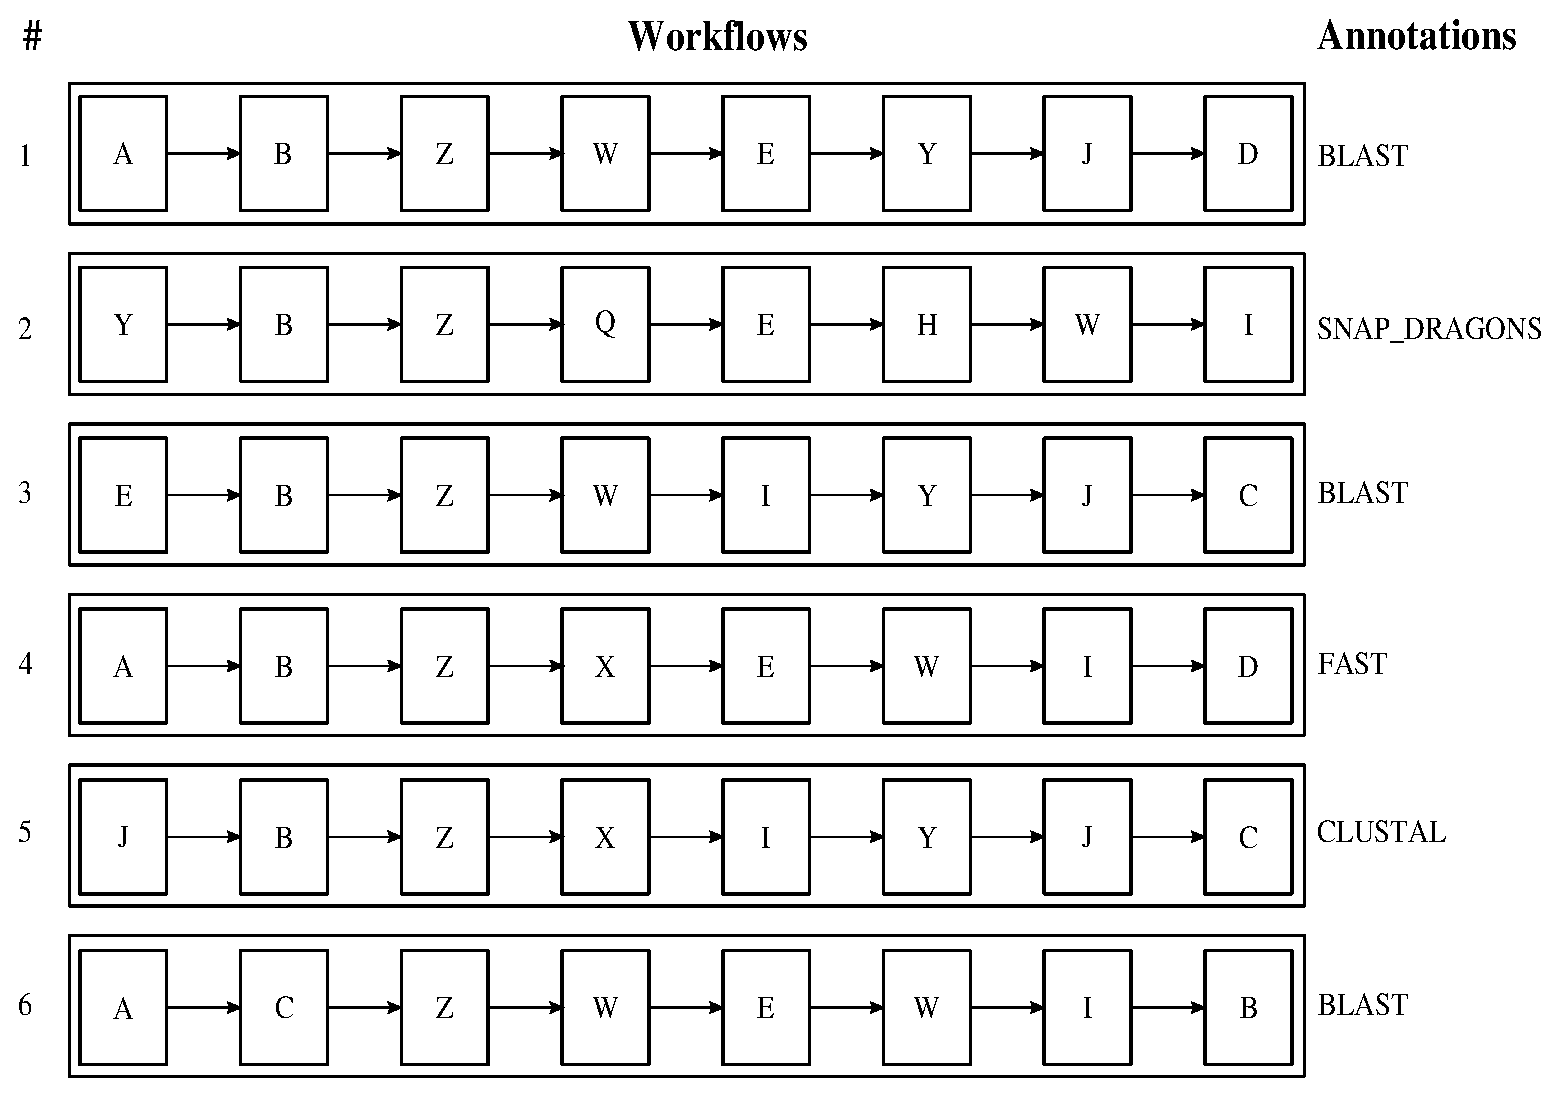
\includegraphics[scale = 0.3]{./pics/recomendacaofreqontologia.eps}
	\label{FIGURA_ONTOLOGIA_CONSTRUIDA2}
\end{figure}

The FIOO solution begins by calculating the frequency of occurrence of each pair of existing activities, which is the number of times that an activity \emph{W} occurs immediately after another activity \emph{Z}. By considering only activities that have already been connected (on the dataset of workflows), the output and input compatibility is guaranteed.

After calculating the frequency, it is necessary to annotate all the workflows of the figure~\ref{FIGURA_ONTOLOGIA_CONSTRUIDA2}, using the concepts of the domain ontology (see Figure~\ref{FIGURA_ONTOLOGIA_CONSTRUIDA}). This step was performed manually. Finally, the algorithm annotates all activities with the same annotations of their respective workflow; i.e., if the \emph{X} activity (Figure \ref{FIGURA_ONTOLOGIA_CONSTRUIDA2}) is inside two workflows with distinct annotations, then this activity will be related to two different concepts from the ontology. The final result is presented in Table \ref{tabela_lista_recomendacao_ordenada_frequencia}, which contains the activities' frequencies and annotations.
\begin{figure}[!htb]
	\centering
	\caption{{\bf Ontology.} Ontology built to annotate scientific workflows with ontological concepts.}
	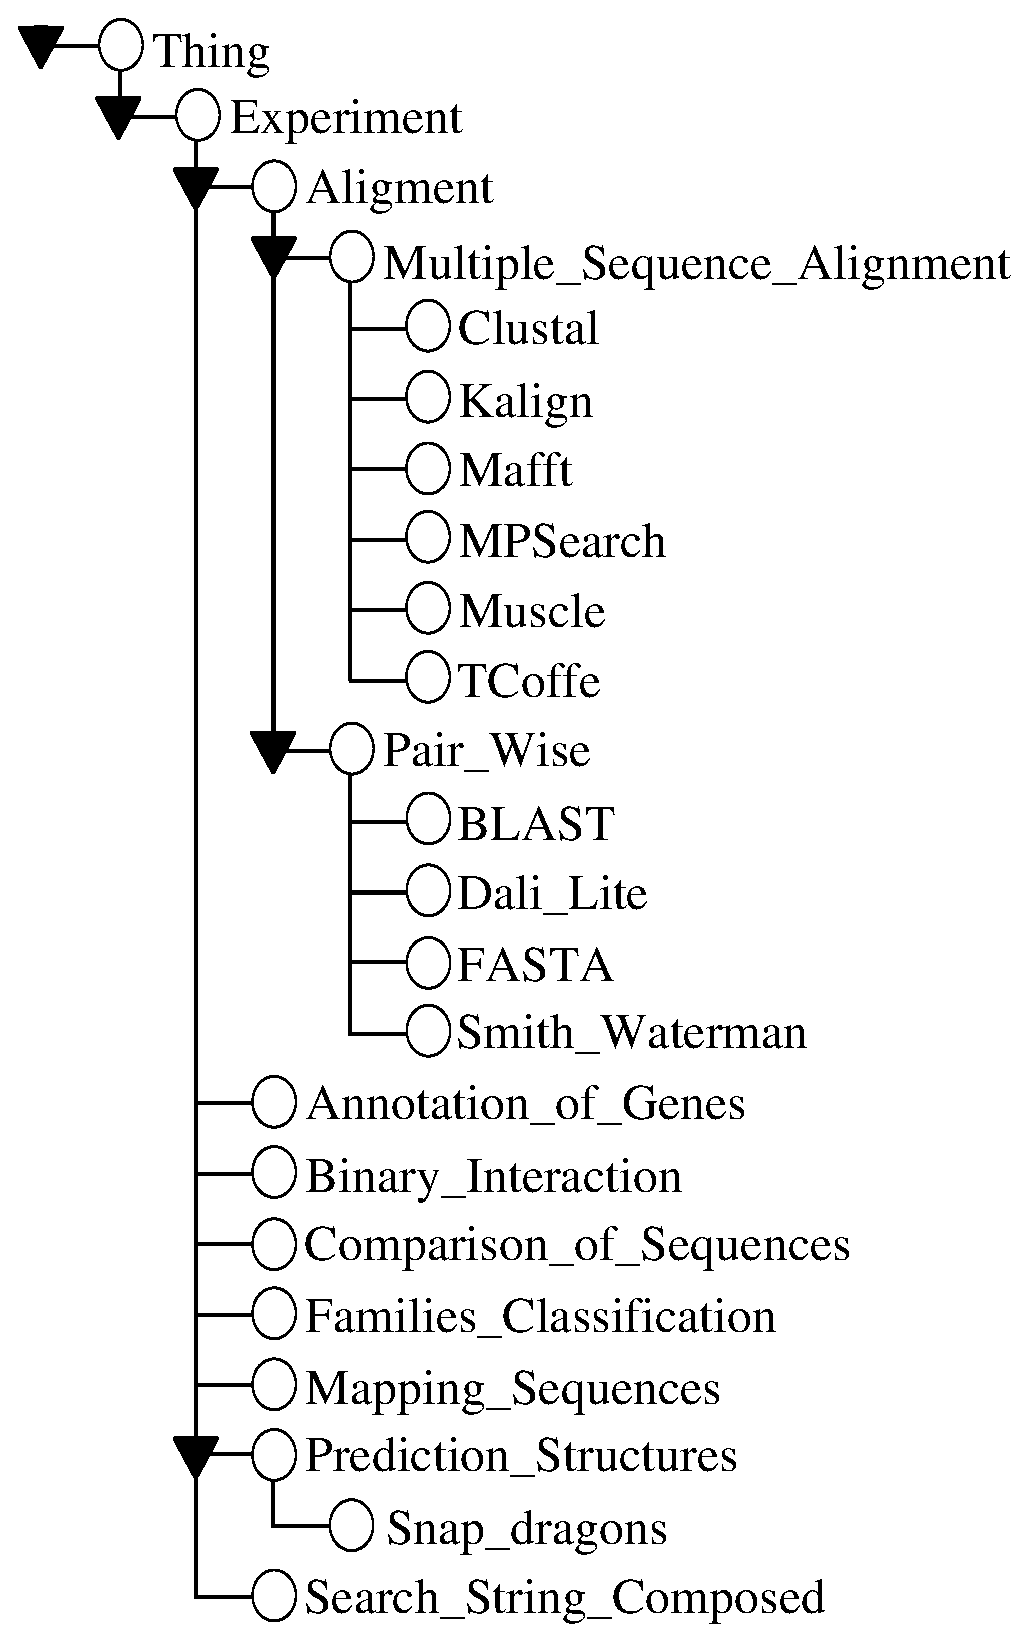
\includegraphics[scale = 0.3]{./pics/ontologia.eps}
	\label{FIGURA_ONTOLOGIA_CONSTRUIDA}
\end{figure}

To understand the recommendation training mechanism, another example will be used to simulate a user interacting with the recommendation system. Let us assume that during the construction of the workflow~\(1\) (see Figure~\ref{FIGURA_ONTOLOGIA_CONSTRUIDA}) a scientist inserts the \emph{Z} activity and asks for a recommendation. The system will look at the list of activities that occurs after \emph{Z} sorted by frequency and ontological concept and will return the recommendation list presented in table~\ref{tabela_lista_recomendacao_ordenada_frequencia}. The sorting considering the ontological concepts serves as a tiebreaker criterion when two activities have the same frequency. In this example, according to the recommendation list of Table~\ref{tabela_lista_recomendacao_ordenada_frequencia}, the \emph{W} activity would be first recommended to the user.


\begin{table}[!htb]
	\tiny
	\centering
	\caption{Recommendation for activity \emph{Z} sorted by frequency and ontological concept}
	\begin{tabular}{|c|c|c|c|}  \hline
		\textbf{Position} & \textbf{Activ} & \textbf{Frequency} & \textbf{Annotation} 	\\ \hline
		1				& W 				& 3 				& BLAST				\\ \hline
		2				& X 				& 2 				& FAST, CLUSTAL		\\ \hline
		3				& Q 				& 1 				& SNAP DRAGONS		\\ \hline
		\(\vdots\)		& \(\vdots\)		& \(\vdots\) 		& \(\vdots\)		\\ \hline
		280				& \(\vdots\)		& \(\vdots\)		& \(\vdots\)	\\ \hline
	\end{tabular}
	\label{tabela_lista_recomendacao_ordenada_frequencia}
	\vspace{0.1cm}
\end{table}

The activities are annotated with the same annotation of the workflows that contain them. Thus, it is possible that there is at least one activity with more than one annotation. This creates a new recommendation case to consider. Suppose both \emph{W} and \emph{X} activities contains in their annotation lists the concept \emph{BLAST}. In this case, the activity with a lower number of annotations would be recommended, since it is considered more specific for the experiment in question. If both activities have the same number of annotations, the alphabetical order of concepts is used as the tie-breaking criterion. If a new tie occurs a random selector is used.

\section*{Results}
Table \ref{tb_resultadosExperimentos} displays the results of each recommendation system used. FIOO corresponds to our Frequency INput Output and Ontology approach. The techniques that have the letter \emph{C} in subscript are classifiers; the ones that have letter \emph{R} in subscript are regressors; and those that have nothing are from related literature. Each system makes its recommendations according to its own criteria in an recommendation list. Then the activities not recommended are added to the end of this list. Thus, the correct activity will always be found, and the factor that differentiates the recommendation systems is the position the activities are in the recommendation list, which contains \(280\) positions.
\bgroup
\begin{table}[!htp]
	%\centering
	\tiny
	\caption{Recommendation results}
	\begin{tabular}{|l|l|l|l|l|l|l|l|} \hline
		\tiny
		\textbf{\(\mathbf{\#}\)} & \textbf{Approach}&\textbf{S@1}&\textbf{S@5} & \textbf{S@50} & \textbf{S@100} & \textbf{S@280} & \textbf{MRR} \\ \hline
		
		1  & Random					& 0,00 & 0,02 & 0,03 & 0,04 & 1 & 0,033 \\ \hline
		2  & \emph{Apriori}			& 0,00 & 0,03 & 0,05 & 0,05 & 1 & 0,037 \\ \hline
		3  & KNN\(_C\)				& 0,00 & 0,06 & 0,50 & 1,00 & 1 & 0,040 \\ \hline
		4  & N. Network\(_C\)		& 0,01 & 0,15 & 0,80 & 1,00 & 1 & 0,089 \\ \hline
		5  & CART\(_C\)				& 0,02 & 0,12 & 0,76 & 1,00 & 1 & 0,113 \\ \hline
		6  & CART\(_R\)    			& 0,13 & 0,13 & 0,61 & 1,00 & 1 & 0,114 \\ \hline
		7  & Naive Bayes\(_C\)     	& 0,02 & 0,15 & 0,63 & 1,00 & 1 & 0,114 \\ \hline
		8  & Binomial\(_R\) 		& 0,08 & 0,19 & 0,84 & 1,00 & 1 & 0,136 \\ \hline
		9  & N. Network\(_R\)   	& 0,10 & 0,26 & 0,26 & 1,00 & 1 & 0,154 \\ \hline
		10 & MARS\(_R\)     		& 0,12 & 0,20 & 0,72 & 1,00 & 1 & 0,167 \\ \hline
		11 & FIO           			& 0,14 & 0,26 & 0,86 & 1,00 & 1 & 0,196 \\ \hline
		12 & SVM\(_R\)     			& 0,12 & 0,31 & 0,84 & 1,00 & 1 & 0,238 \\ \hline
		13 & SVM\(_C\)    			& 0,24 & 0,46 & 0,71 & 1,00 & 1 & 0,244 \\ \hline
		14 & Comp. SVM\(_C\)		& 0,25 & 0,44 & 0,76 & 1,00 & 1 & 0,314 \\ \hline
		15 & Rot. Forest\(_C\)  	& 0,29 & 0,45 & 0,77 & 1,00 & 1 & 0,324 \\ \hline
		16 & FIOO          			& 0,34 & 0,46 & 0,81 & 1,00 & 1 & 0,334 \\ \hline
	\end{tabular}
	\label{tb_resultadosExperimentos}
	\vspace{0.1cm}
\end{table}
\egroup


The \emph{Random} approach did not require training. The algorithm only randomly selected activities, forming a list of recommended activities. This system recommended less than \(3\%\) of the correct activities in the top ten positions. Most of the correct activities were rated close to position \(140\) which is the average position of the recommended lists. The metric values ​​\(S@280 = 1\) and \(S@100 = 0.04\) indicate that most of the correct items were found after the hundredth position. This system was used to calculate the simplest baseline.

The system using the \emph{Apriori} technique achieved its best performance when the \emph{confidence} and \emph{support} parameters were defined as \emph{without limitation}, that means, no minimum confidence and support values were defined for the creation of association rules. All rules were considered valid. Even without restricting these values, the results of this technique presented results better than only the \emph{Random} approach. Recommending less than \(6\%\) of correct activities between the \(50\) first positions, its accuracy is still low with the value of \(MRR = 0.037\). The poor results of this technique happened due to the fact the technique disregards the order of the activities during the generation of the rules and, consequently, of the recommendation.

The \emph{KNN}  based approach has been trained considering different values ​​of the parameter \emph{k} (from 1 to 100) which represents the number of nearest neighbours (and using the Euclidean distance as the proximity metric). The best recommendation results for this approach were obtained with \(k = 2\). Even so, less than \(10​​\%\) of the correct items were found among the top ten items in the list and \(50\%\) of items in the first 50 items. According to the MRR metric, the average position of the recommended items was far from the first position in the list (\(MRR = 0.04\)). These results indicate that classifying activities according to the distance between groups of neighbours is not an appropriate approach to this problem.

The approach which uses an MLP neural network as a classifier had results significantly better than the ones achieved by the \emph{KNN} approach when considering the metric S@1 (\(0.0137\) versus \(0.0037\)). For the training of the network the parameters used were: i) number of neurons \(\eta\) (ranging from \(1:40\)); ii) learning rate \(\alpha\) (ranging from \(10^{-7}: 10\)); iii) two hidden layers; and iv) fully connected architecture. The best classification results were achieved with \(\eta = 18\) and \(\alpha = 10^{-4}\), obtaining \(17\%\) of items ranked among the top ten positions in the list, and \(80\%\) among the \(50\) first positions, which represents an improvement of \(30\%\) when compared with the \emph{KNN} approach. The metric value \(MRR = 0.089\) was twice as high as the one from \emph{KNN}, this growth in precision indicates the neural network generalization power to solve non-linear problems was more efficient than the previous approaches.

The approach which uses CART as a classifier, dealing with categorical data, presented a result superior to the one from neural network. The training used the parameters: i) minimum division value \(\gamma = [0:30]\); ii) maximum final tree size \(\delta = [0:10000]\); iii) minimum variation value to perform a division \(cp = [10^{-7}:10]\); iv) division function (\(\xi\)) as Gini Index or Information Gain. The best result was achieved with \(gamma = 0\), \(\delta = 30\), \(cp = 10^{-3} \), and \(\xi = \) Information Gain.

The results of this approach were approximately twice as good as those of the neural network. This indicates approaches that deal with categorical data by nature has a potential for obtaining good results in problems such the one treated in this paper. The MRR results were \(26\%\) better than the ones achieved by the MLP based approach, and this approach was able to recommend \(12.3\%\) of the searched items in the first position and 76\% in the first \(50\) positions.

The approach which uses CART as regressor achieve its best results with \(gamma = 2\), \(\delta = 20\), \(cp = 10^{-5}\), and \(\xi = \)Information Gain. The recommendation that used continuous values ​​presented a result superior to \(CART_C\) considering the metrics \(S@1\) and \(S@5\) and worse results for \(S@10\) and \(S@50\). The general precision (MRR) of \(CART_R\) was slightly higher than the one achieved by \(CART_C\).



%O sistema baseado no classificador Naive Bayes obteve resultados muito próximos ao do regressor CART. O treinamento ocorreu modificando o atributo \emph{correção de Laplace} com valores entre \([0:100]\). O melhor resultado ocorreu para o valor zero obtendo \(34\%\) dos itens recomendados entre as dez primeiras posições e \(63\%\) entre as \(50\) primeiras posições. Em contrapartida, o valor de \(MRR\) não sofreu grande variação.
%
%O sistema baseado em regressor binomial apresentou melhoria em relação ao Naive Bayes e à rede neural (técnicas que apresentaram resultados próximos). O treinamento dessa técnica ocorre por máxima verossimilhança de um modelo generalizado linear aproximado por uma distribuição binomial. Os resultados para \(S@5\) e \(S@50\) foram superiores que das técnicas anteriores e o valor da métrica \(MRR\) melhorou em aproximadamente \(19\%\) em relação a técnica Naive Bayes. Isto indica que aproximar a variável dependente por uma distribuição binomial e estimar seus parâmetros por verossimilhança é uma ideia potencialmente interessante para tratar este problema.
%
%A rede neural como regressor, que utiliza o peso da rede neural como saída, foi treinada de forma análoga à rede neural usada como classificador. O melhor resultado foi obtido para os valores de \(\eta = 10\) e \(\alpha = 10^{-2}\) recomendando \(26\%\) dos itens corretos entre as dez primeiras posições da lista. A precisão do sistema (MRR) melhorou \(13\%\) em relação ao regressor binomial. Esses resultados indicam que usar um regressor ao invés de um classificador apresenta um resultado melhor para esse tipo de problema, quando solucionado com redes neurais.
%
%O sistema que usou o algoritmo MARS como regressor apresentou um resultado superior à rede neural (usada como regressor) em \(12,5\%\) na métrica \(S@1\), três vezes mais atividades recomendadas entre as \(50\) primeiras e um aumento de precisão geral (MRR) de \(8\%\). Esse resultado mostra que as curvas criadas pelas diversas funções conectadas do MARS obtiveram uma generalização melhor que da rede neural. O treinamento dos parâmetros foi por verossimilhança.
%
%O regressor SVM apresentou resultados duas vezes melhores que o algoritmo MARS para a medida S@10, pois em \(49\%\) das recomendações o item correto estava entre as dez primeiras posições da lista de recomendações. O valor de MRR também foi superior (\(42\%\)). O treinamento foi feito por otimização de margem com os valores de \(c = [10^{-7}:10^{2}]\) , \(\epsilon = [10^{-7}:10^{2}]\), valores de tolerância \(\beta = [10^{-7}:10^{2}]\), funções de \emph{kernel}: i) linear; ii) sigmoide; iii) polinomial; e iv) radial, os parâmetros do \emph{kernel} polinomial são: i) \(p = [1:10]\) que é a potência da função. Os melhores valores encontrados foram para \(c = 1\), \(\epsilon = 1\), \(\beta = 10^{-4}\), \emph{kernel} polinomial com \(p = 2\). Esse resultado é um indício que o problema não é linearmente separável, pois foi usada uma função de \emph{kernel} polinomial para mapear o problema em alta dimensão e projetá-lo novamente para uma dimensão mais baixa. Os autores acreditam que esta característica foi responsável pelo bom desempenho desse regressor.
%
%Dentre os sistemas propostos pela literatura, o sistema baseado em entrada, saída e frequência (FES) \cite{Wang2008} é o que apresenta os melhores resultados. Nos experimentos realizados, este sistema identificou o item correto entre as dez primeiras posições da lista de recomendação em \(37\%\) dos casos, e obteve um valor de \(MRR = 0,196\).
%
%O sistema baseado no algoritmo SVM para classificação foi o único classificador que superou os resultados dos regressores. Seu treinamento foi análogo ao SVM para regressão. Sua melhor execução foi para os valores \(c = 10^{-1}\), \(p = 10^{-4}\) e \emph{kernel} linear. Esta execução, para a métrica \(S@1\) foi \(64\%\) melhor que a da técnica FES e o valor da precisão geral (MRR) aumentou \(24\%\). Este resultado indica que a solução utilizando \emph{kernel} para mapeamento em alta dimensão é uma proposta eficiente no caso de classificadores.
%
%O sistema SVM composto, que executa sobre os resultados dos outros sistemas de recomendação, apresentou um desempenho superior ao SVM para classificação. Seu treinamento foi análogo ao do SVM\(_{C}\) e seu melhor desempenho foi para os parâmetros \(c = 10^{-2}\), \(p = 1\) e \emph{kernel polinomial}. Houve uma melhoria de \(3\%\) na métrica \(S@1\) e \(28\%\) na métrica \(MRR\), essa melhoria é em virtude do uso do resultado de outros classificadores em conjunto com a redução de esparsidade do conjunto de dados.

%O sistema utilizando \emph{Rotation Forest} apresentou o segundo melhor resultado, seu treinamento utilizou os parâmetros: i) valor mínimo de divisão \(\gamma = [0:30]\); ii) tamanho máximo da árvore final \(\delta = [0:10000]\) ; iii) valor mínimo de variação para realizar uma divisão \(cp = [10^{-7}:10^{+1}]\); iv) função de divisão (\(\xi\)) como índice de Gini e ganho de informação; v) \(K = [1:10]\) como número de partições; vi) \(L = [1:10]\) como o número de classificadores; e vii) valores de corte \(0,25; 0,5; 0,75\). Essa melhoria foi em virtude de usar em conjunto uma técnica de classificação do tipo \emph{ensemble} e três limiares de corte, os quais foram estabelecidos para converter os valores numéricos (da média dos \(L\) classificadores) em valores binários.
%
%A técnica FESO, apresentou um resultado superior às demais. Este  considera o uso de frequência, entrada e saída e informações semânticas sobre as atividades. Em comparação com as demais técnicas seu resultado foi superior para todas as métricas calculadas, exceto \(S@50\) para algumas técnicas. Em relação à técnica FES, seu resultado foi superior. Em particular, parte dessa melhora é justificada pelos casos em que a atividade correta teria frequência zero no conjunto de treinamento, pois ela permite recomendar baseada na ontologia (usando as atividades que contenham a ontologia do novo workflow). Além disso, para o caso em que há empate entre duas atividades com o critério de entrada e saída e a frequência a técnica proposta apresenta um fator a mais para ser utilizado como desempate.
%
%Algumas tendências observadas com esses resultados foram que aumentar a informação sobre dados na recomendação melhora o seu desempenho, como o resultado dos experimentos: 2, 12 e 14 mostram. Uma segunda tendência é que o classificador SVM foi o único que obteve um melhor resultado que os regressores, indicando que soluções por maximização de espaço entre dados em alta dimensão podem ser uma área de estudo promissora. Uma terceira tendência é o uso de classificadores compostos e \emph{ensembles}, os quais apresentaram resultados promissores. No caso do \emph{ensemble} há um indício que técnicas desse tipo, que usem limiares para converter os valores da média dos resultados do conjunto \(L\) em valores binários, têm resultados promissores na recomendação de atividades.






%\section*{Discussion}
%DISCUSSAO
%Nulla mi mi, venenatis sed ipsum varius, Table~\ref{table1} volutpat euismod diam. Proin rutrum vel massa non gravida. Quisque tempor sem et dignissim rutrum. Lorem ipsum dolor sit amet, consectetur adipiscing elit. Morbi at justo vitae nulla elementum commodo eu id massa. In vitae diam ac augue semper tincidunt eu ut eros. Fusce fringilla erat porttitor lectus cursus, vel sagittis arcu lobortis. Aliquam in enim semper, aliquam massa id, cursus neque. Praesent faucibus semper libero~\cite{bib3}.

The Naive Bayes classifier based approach obtained results very similar to the ones achieved by the CART regressor. The training occurred by ranging the \emph{Laplace correction} attribute with values ​​between \([0:100]\). The best result occurred with value zero for this parameter, achieving \(34\%\) of the recommended items in the top ten positions and \(63\%\) among the first \(50\) positions. In contrast, the value of \(MRR\) did not change much.

The binomial regressor approach presented better results when compared with the Naive Bayes and the neural network approaches. The training of this technique occurs using the maximum likelihood for a generalized linear model approximated by a binomial distribution. The results for \(S@5\) and \(S@50\) were higher than the achieved by the previous approaches and the value of the metric \(MRR\) improved by approximately 19\% when compared to the one achieved by the Naive Bayes approach.

The approach which uses a neural network as regressor, considering the weight of the neural network as output, was trained in an analogous way to the neural network used as a classifier. The best result was obtained for the values ​​of \(\eta = 10\) and \(\alpha = 10^{-2}\). It was able to recommend \(26\%\) of the correct items among the top ten positions in the list. System accuracy (MRR) improved \(13\%\) from the achieved by the binomial regressor. These results indicate that using a regressor instead of a classifier presents a better result for this kind of problem, at least when using neural networks.

The approach based on the MARS algorithm as regressor achieved a better result than the one from the neural network (used as regressor). The metric \(S@1\) was improved in \(12.5\%\) and the overall precision (MRR) increased  \(8\%\). This result shows that the curves created by the various connected functions of the MARS obtained a better generalization than the neural network. The training of the parameters was performed using likelihood.

Among the systems proposed in the literature, the system based on input, output and frequency (FIO) (\cite{Wang2008}) is the one with the best results. In the experiments performed, this system identified the correct item among the top ten positions of the recommendation list in \(37\%\) of the cases, and obtained a value of \(MRR = 0.196\).

The SVM regressor presented results twice as good as the MARS algorithm for the metric \(S@10\), since in \(49\%\) of the recommendations the correct item was among the top ten positions in the recommendations list. The MRR value was also higher (\(42\%\)). The training was performed using margin optimization with the values ​​of \(c = [10^{-7}:10^2]\), \(\epsilon = [10^{-7}:10^{2}]\), Tolerance values ​​\(\beta = [10^{-7}:10^{2}]\),  kernel functions: i) linear; ii) sigmoid; iii) polynomial; and (iv) radial. The tested values of the parameter of the polynomial kernel were  \(p = [1:10]\) which is the power of the function. The best results were achieved for \(c = 1\), \(\epsilon = 1\), \(\beta = 10^{-4}\), and polynomial kernel with \(p = 2\). %The fact that the best results obtained with a polynomial kernel is a clue that the problem is not linearly separable, since a polynomial kernel function was used to map the problem to high dimension and project it back to a smaller dimension. The authors believe that this characteristic was responsible for the good performance of this regressor.

The approach based on the SVM algorithm for classification was the only classifier that surpassed the results of the regressors. His training was analogous to the SVM for regression. Its best results were achieved with ​\(c = 10^{-1}\), \(p = 10^{-4}\), and \emph{linear kernel}. The value of the metric \(S@1\) was \(64\%\) better than the one from FIO technique and the general precision value (MRR) increased \(24\%\). This result indicates that the solution using \emph{kernel} for high-dimensional mapping is an efficient approach in the case of classifiers.

The composed SVM system, which recommends items based on the results of the other recommendation approaches, achieved better results than the SVM. Its training was analogous to that of SVM\(_C\) and its best results were achieved with \(c = 10^{-2}\), \(p = 1\), and polynomial kernel. There was an improvement of \(3\%\) in the metric \(S@1\) and \(28\%\) in the metric \(MRR\), this improvement is due to the use of the result of other classifiers together with the sparsity reduction of the data set.

The system using \emph{Rotation Forest} presented the second best result, its training used the parameters: i) minimum division value \(\gamma = [0:30]\); ii) maximum final tree size \(\delta = [0:10000]\); iii) minimum variation value to perform a division \(cp = [10^{-7}:10]\); iv) division function (\(\xi\)) using Gini Index and Information Gain; v) \(K = [1:10]\) as the number of partitions; vi) \(L = [1:10]\) as the number of classifiers; and (vii) cutoff values ​​\(0.25, 0.5, 0.75\). Is use of an ensemble classification technique was able to achieve better results, for example, \(S@1 = 0.29\), \(S@10 = 0.54\), and \(MRR = 0.324\).

Our ontology-based approach (FIOO) achieved better (or at least equal) results than the previous approaches for almost all of the evaluated metrics. It considers the use of frequency, input, output, and semantic information about the activities. In comparison to the other techniques, its result was higher for all calculated metrics, except \(S@50\) for some techniques. In relation to the FIO technique, its result was superior. In particular, part of this improvement is justified by cases where the correct activity has zero frequency in the training set. Since FIOO considers the ontology information it is able to recommend activities even if they have zero frequency in the train set. In addition, for the case where there is a tie between two activities considering the input, output, and the frequency criteria, the proposed technique presents an additional factor to be used as a tie breaker.

We were able to identify some trends in these results. Increasing information on data in the recommendation improves the recommenders performance, as the result of the experiments: 2, 12, and 14 show. A second trend is that the SVM classifier was the only one that obtained a better result than the regressors, indicating that solutions by maximizing space between data in high dimension may be a promising area of ​​study. A third trend is the use of composite classifiers and \emph{ensembles}, which presented promising results. In the case of the \emph{ensemble}, there is a clue that techniques of this kind, which use thresholds to convert the mean values ​​of the set result \(L\) into binary values, have promising results in recommending activities.

\section*{Conclusions}
This work presented a hybrid approach to recommend activities in scientific workflows, called FIOO. It uses syntax compatibility, frequency, and domain ontology to recommend activities. We also modelled the problem of recommendation as an artificial intelligence classification and regression problem. 

Our results were compared with the ones presented in the related literature which was previously identified through a systematic literature review. In this review, we identified techniques, their restrictions, their advantages and the forms that they were validated. 

In order to perform the comparison, a relational database of workflows and their activities was constructed. It was also necessary to establish a methodology to compare different activity recommendation techniques for the same data set with the same validation metrics (\(S@k\) and \(MRR\)).

When comparing all techniques, certain aspects of the data set were verified, such as the fact that the activities were not independent; the problem is not linearly separable, and that clustering techniques were not adequate to solve this problem. With the exception of SVM, regressors presented more accurate results than classifiers. Finally, adding information in the recommendation systems improved their accuracy.

As future works, we intend to investigate the use of data provenance to increase the accuracy of the recommendations.


%\section*{Acknowledgement}
%The project is funded in part by the National Institutes of Health, under Grant No. 5R01CA136535.


%%%%%%%%%%%%%%%%%%%%%%%%%%%%%%%%%%%%%%%%%%%%%%%%%%%%%%%%%%%%%%%%%%%%%%%%%%%%%%%%%%%%%

%\bibliography{ijmso}
%\bibliographystyle{unsrt}
%\bibliographystyle{alpha}

\begin{thebibliography}{10}

%	\bibitem{BeautifulSoup2015}
%	Richardson L. Beautiful Soup; 2015.
%	\newblock Available from: \url{http://www.crummy.com/software/BeautifulSoup/}.
\bibitem[\protect\citeauthoryear{BeautifulSoup}{BeautifulSoup (2015)}]{BeautifulSoup2015}
BeautifulSoup; http://www.crummy.com/software/BeautifulSoup/

%\bibitem{Biocatalogue}
%Bhagat J, Tanoh F, Nzuobontane E, Laurent T, Orlowski J, Roos M, et~al..
%BioCatalogue: a universal catalogue of web services for the life sciences;
%2014.
%\newblock Available from: \url{doi:10.1093/nar/gkq394}.
\bibitem[\protect\citeauthoryear{BioCatalogue}{BioCatalogue (2015)}]{BioCatalogue2015}
BioCatalogue: a universal catalogue of web services for the life sciences; https://www.ncbi.nlm.nih.gov/pubmed/20484378


%\bibitem{Bomfim2005}
%Bomfim E, Oliveira J, de~Souza JM, Strauch J.
%\newblock Thoth: improving experiences reuses in the scientific environment
%through workflow management system.
%\newblock In: Computer Supported Cooperative Work in Design, 2005. Proceedings
%of the Ninth International Conference. vol.~2; 2005. p. 1164--1170 Vol. 2.
%\newblock Available from:
%\url{http://ieeexplore.ieee.org/xpl/articleDetails.jsp?arnumber=1504261}.
\bibitem[\protect\citeauthoryear{Bomfim E, Oliveira J, de~Souza JM, Strauch J.}{2005}]{Bomfim2005}
Bomfim E, Oliveira J, de~Souza JM, Strauch J. {2005} 'Computer Supported Cooperative Work in Design, 2005. Proceedings
of the Ninth International Conference.' vol.~2; 2005. p. 1164--1170 Vol. 2.


%\bibitem{Cao2012}
%Cao B, Yin J, Deng S, Wang D, Wu Z.
%\newblock Graph-based workflow recommendation: on improving business process
%modeling.
%\newblock In: Proceedings of the 21st ACM international conference on
%Information and knowledge management. CIKM '12. ACM; 2012. p. 1527--1531.
%\newblock Available from: \url{http://doi.acm.org/10.1145/2396761.2398466}.
\bibitem[\protect\citeauthoryear{Cao B, Yin J, Deng S, Wang D, Wu Z.}{2012}]{Cao2012}
Cao B, Yin J, Deng S, Wang D, Wu Z. {2012} 'Proceedings of the 21st ACM international conference on
Information and knowledge management. CIKM '12. ACM; 2012. p. 1527--1531.


%	\bibitem{Cerezo2011}
%	Cerezo N, Montagnat J.
%	\newblock {Scientific Workflow Reuse Through Conceptual Workflows on the
%		Virtual Imaging Platform}.
%	\newblock In: Proceedings of the 6th Workshop on Workflows in Support of
%	Large-scale Science. \{WORKS\} '11. ACM; 2011. p. 1--10.
%	\newblock Available from: \url{http://doi.acm.org/10.1145/2110497.2110499}.
\bibitem[\protect\citeauthoryear{Cerezo N, Montagnat J.}{2011}]{Cerezo2011}
Cerezo N, Montagnat J. {2011} 'Proceedings of the 6th Workshop on Workflows in Support of
Large-scale Science. \{WORKS\} '11. ACM; 2011. p. 1--10.'


%\bibitem{Diamantini2012}
%Diamantini C, Potena D, Storti E.
%\newblock {Mining Usage Patterns from a Repository of Scientific Workflows}.
%\newblock In: Proceedings of the 27th Annual \{ACM\} Symposium on Applied
%Computing. SAC '12. ACM; 2012. p. 152--157.
%\newblock Available from: \url{http://doi.acm.org/10.1145/2245276.2245307}.
\bibitem[\protect\citeauthoryear{Diamantini C, Potena D, Storti E.}{2012}]{Diamantini2012}
Diamantini C, Potena D, Storti E. {2012} 'Proceedings of the 27th Annual \{ACM\} Symposium on Applied
Computing. SAC '12. ACM; 2012. p. 152--157.


%\bibitem{Garijo2013}
%Garijo D, Corcho O, Gil Y.
%\newblock {Detecting Common Scientific Workflow Fragments Using Templates and
%	Execution Provenance}.
%\newblock In: Proceedings of the Seventh International Conference on Knowledge
%Capture. K-CAP '13. New York, NY, USA: ACM; 2013. p. 33--40.
%\newblock Available from: \url{http://doi.acm.org/10.1145/2479832.2479848}.
\bibitem[\protect\citeauthoryear{Garijo D, Corcho O, Gil Y.}{2013}]{Garijo2013}
Garijo D, Corcho O, Gil Y. {2013} 'Proceedings of the Seventh International Conference on Knowledge
Capture. K-CAP '13. New York, NY, USA: ACM; 2013. p. 33--40.


%	\bibitem{CorchoGarijo2014}
%	Garijo D, Corcho O, Gil Y, Braskie MN, Hibar D, Hua X, et~al.
%	\newblock {Workflow Reuse in Practice: A Study of Neuroimaging Pipeline Users}.
%	\newblock Proceedings of the 2014 IEEE 10th International Conference on
%	eScience. 2014; p. 239--246.
\bibitem[\protect\citeauthoryear{Garijo D, Corcho O, Gil Y, Braskie MN, Hibar D, Hua X, et~al.}{2014}]{CorchoGarijo2014}
Garijo D, Corcho O, Gil Y, Braskie MN, Hibar D, Hua X, et~al. {2014} 'Proceedings of the 2014 IEEE 10th International Conference on
eScience.' 2014; p. 239--246.


%@Article{Harvey2010,

%	Title                    = {{Ranking Social Bookmarks Using Topic Models}},

%	Author                   = {Harvey, Morgan and Ruthven, Ian and Carman, Mark},

%	Journal                  = {Proceedings of the 19th ACM International Conference on Information and Knowledge Management},

%	Year                     = {2010},

%	Pages                    = {1401--1404},

%	Url                      = {http://doi.acm.org/10.1145/1871437.1871632}

%}
\bibitem[\protect\citeauthoryear{Harvey, Morgan and Ruthven, Ian and Carman, Mark}{2010}]{Harvey2010}
Harvey, Morgan and Ruthven, Ian and Carman, Mark {2010} 'Proceedings of the 19th ACM International Conference on Information and Knowledge Management' 2010; p. 1401--1404.



%\bibitem{Koop2008}
%Koop D.
%\newblock VisComplete: Automating Suggestions for Visualization Pipelines.
%\newblock IEEE Transactions on Visualization and Computer Graphics.
%2008;14(6):1691--1698.
\bibitem[\protect\citeauthoryear{Koop D.}{2008}]{Koop2008}
Koop D. {2008} 'IEEE Transactions on Visualization and Computer Graphics', {\it IEEE}, pp.1691--1698


%\bibitem{Leng2010}
%Leng Y, El-Gayyar M, Cremers AB.
%\newblock {Semantics Enhanced Composition Planner for Distributed Resources}.
%\newblock In: 2010 Ninth International Symposium on Distributed Computing and
%Applications to Business, Engineering and Science. IEEE; 2010. p. 61--65.
%\newblock Available from:
%\url{http://ieeexplore.ieee.org/lpdocs/epic03/wrapper.htm?arnumber=5573302}.
\bibitem[\protect\citeauthoryear{Leng Y, El-Gayyar M, Cremers AB.}{2010}]{Leng2010}
Leng Y, El-Gayyar M, Cremers AB. {2010} 'Ninth International Symposium on Distributed Computing and
Applications to Business, Engineering and Science.' IEEE; 2010. p. 61--65.


%	\bibitem{Mohan2015}
%	Mohan A, Ebrahimi M, Lu S.
%	\newblock 2015 IEEE International Conference on Services Computing A
%	Folksonomy-Based Social Recommendation System for Scientific Workflow Reuse.
%	2015;.
\bibitem[\protect\citeauthoryear{Mohan A, Ebrahimi M, Lu S.}{2015}]{Mohan2015}
Mohan A, Ebrahimi M, Lu S. {2015} 'IEEE International Conference on Services Computing A
Folksonomy-Based Social Recommendation System for Scientific Workflow Reuse'.

	
%	\bibitem{ROURE2015}
%	Roure CG. myExperiment; 2015.
%	\newblock Available from: \url{http://www.myexperiment.org/}.
\bibitem[\protect\citeauthoryear{myExperiment}{myExperiment (2015)}]{ROURE2015}
myExperiment, http://www.myexperiment.org/


%\bibitem{Oliveira2008}
%de Oliveira FT, Murta L, Werner C, Mattoso M.
%\newblock Using Provenance to Improve Workflow Design.
%\newblock In: Freire J, Koop D, Moreau L, editors. Provenance and Annotation of
%Data and Processes. vol. 5272 of Lecture Notes in Computer Science. Springer
%Berlin Heidelberg; 2008. p. 136--143.
%\newblock Available from:
%\url{http://dx.doi.org/10.1007/978-3-540-89965-5\_15}.
\bibitem[\protect\citeauthoryear{Oliveira FT, Murta L, Werner C, Mattoso M.}{2008}]{Oliveira2008}
Oliveira FT, Murta L, Werner C, Mattoso M. {2008} 'Provenance and Annotation of
Data and Processes.' vol. 5272 of Lecture Notes in Computer Science. Springer
Berlin Heidelberg; 2008. p. 136--143.


%	\bibitem{Oliveir2010}
%	de~Oliveira FT.
%	\newblock UM SISTEMA DE RECOMENDAÇÃO PARA COMPOSIÇÃO DE WORKFLOWS.
%	\newblock UNIVERSIDADE FEDERAL DO RIO DE JANEIRO; 2010.
\bibitem[\protect\citeauthoryear{Oliveira FT.}{2012}]{Oliveir2010}
Oliveira FT. {2010} UM SISTEMA DE RECOMENDAÇÃO PARA COMPOSIÇÃO DE WORKFLOWS.; UNIVERSIDADE FEDERAL DO RIO DE JANEIRO; 2010.


%\bibitem{TostaBraganholo2015}
%Oliveira FTd, Braganholo V, Murta L, Mattoso M.
%\newblock {Improving workflow design by mining reusable tasks}.
%\newblock Journal of the Brazilian Computer Society. 2015;21(1):16.
\bibitem[\protect\citeauthoryear{Oliveira FTd, Braganholo V, Murta L, Mattoso M.}{2015}]{TostaBraganholo2015}
Oliveira FTd, Braganholo V, Murta L, Mattoso M. {2015} 'Journal of the Brazilian Computer Society 2015'


%	\bibitem{wget2015}
%	Scrivano G, Niksic H. GNU Wget Introduction to GNU Wget; 2015.
%	\newblock Available from: \url{http://www.gnu.org/software/wget/}.
\bibitem[\protect\citeauthoryear{wget}{Scrivano(2015)}]{wget2015}
Introduction to GNU Wget; http://www.gnu.org/software/wget/


%\bibitem{Shao2007}
%Shao Q, Kinsy M, Chen Y.
%\newblock {Storing and Discovering Critical Workflows from Log in Scientific
%	Exploration}.
%\newblock In: 2007 IEEE Congress on Services (Services 2007). IEEE; 2007. p.
%209--212.
%\newblock Available from:
%\url{http://ieeexplore.ieee.org/lpdocs/epic03/wrapper.htm?arnumber=4278799}.
\bibitem[\protect\citeauthoryear{Shao Q, Kinsy M, Chen Y.}{2007}]{Shao2007}
Shao Q, Kinsy M, Chen Y. {2007} 'IEEE Congress on Services (Services 2007)', {\it IEEE}, pp.209--212


%\bibitem{Shao2009}
%Shao Q, Sun P, Chen Y.
%\newblock {Efficiently discovering critical workflows in scientific
%	explorations}.
%\newblock Future Generation Computer Systems. 2009;25(5):577--585.
\bibitem[\protect\citeauthoryear{Shao Q, Sun P, Chen Y.}{2009}]{Shao2009}
Shao Q, Sun P, Chen Y. {2009} 'Future Generation Computer Systems 2009', {\it IEEE}, pp.577--585


%	\bibitem{Soomro2015}
%	Soomro K, Munir K, Mcclatchey R.
%	\newblock Incorporating Semantics in Pattern-Based Scientific Workflow
%	Recommender Systems. 2015;
\bibitem[\protect\citeauthoryear{Soomro K, Munir K, Mcclatchey R.}{2015}]{Soomro2015}
Soomro K, Munir K, Mcclatchey R. {2015} 'Incorporating Semantics in Pattern-Based Scientific Workflow
Recommender Systems.' 2015;


%\bibitem{Tan2011}
%Tan W, Zhang J, Madduri R, Foster I, {De Roure} D, Goble C.
%\newblock {Providing Map and GPS Assistance to Service Composition in
%	Bioinformatics}.
%\newblock In: 2011 IEEE International Conference on Services Computing. IEEE;
%2011. p. 632--639.
%\newblock Available from:
%\url{http://ieeexplore.ieee.org/lpdocs/epic03/wrapper.htm?arnumber=6009316}.
\bibitem[\protect\citeauthoryear{Tan W, Zhang J, Madduri R, Foster I, {De Roure} D, Goble C.}{2009}]{Tan2011}
Tan W, Zhang J, Madduri R, Foster I, {De Roure} D, Goble C. {2009} 'IEEE International Conference on Services Computing.';
2011. p. 632--639. 


%\bibitem{Telea1999}
%Telea A, van Wijk JJ.
%\newblock Vission: An Object Oriented Dataflow System for Simulation and
%Visualization.
%\newblock In: PROCEEDINGS OF IEEE VISSYM; 1999. p. 95--104.
%\newblock Available from:
%\url{http://link.springer.com/chapter/10.1007%2F978-3-7091-6803-5_21}.
\bibitem[\protect\citeauthoryear{Telea A, van Wijk JJ.}{1999}]{Telea1999}
Telea A, van Wijk JJ. {1999} 'PROCEEDINGS OF IEEE VISSYM'; 1999. p. 95--104.


%\bibitem{Wang2008}
%Wang J, Han Y, Yan S, Chen W, Ji G.
%\newblock VINCA4Science: A Personal Workflow System for e-Science.
%\newblock In: Internet Computing in Science and Engineering, 2008. ICICSE '08.
%International Conference on; 2008. p. 444--451.
%\newblock Available from:
%\url{http://ieeexplore.ieee.org/xpl/articleDetails.jsp?arnumber=4548305}.
\bibitem[\protect\citeauthoryear{Wang J, Han Y, Yan S, Chen W, Ji G.}{2008}]{Wang2008}
Wang J, Han Y, Yan S, Chen W, Ji G. {2008} Internet Computing in Science and Engineering, 2008. ICICSE '08.
International Conference on'; 2008. p. 444--451


%\bibitem{Wang2009}
%Wang Y, Cao J, Li M.
%\newblock {Change Sequence Mining in Context-Aware Scientific Workflow}.
%\newblock In: 2009 IEEE International Symposium on Parallel and Distributed
%Processing with Applications. IEEE; 2009. p. 635--640.
%\newblock Available from:
%\url{http://ieeexplore.ieee.org/lpdocs/epic03/wrapper.htm?arnumber=5207868}.
\bibitem[\protect\citeauthoryear{Wang Y, Cao J, Li M.}{2009}]{Wang2009}
Wang Y, Cao J, Li M. {2009} 'IEEE International Symposium on Parallel and Distributed
Processing with Applications.'; 2009. p. 635--640.


%\bibitem{Wang2010}
%Wang F, Deng H, Guo L, Ji K.
%\newblock {A Survey on Scientific Workflow Techniques for Escience in
%	Astronomy}.
%\newblock In: 2010 International Forum on Information Technology and
%Applications. vol.~1. IEEE; 2010. p. 417--420.
%\newblock Available from:
%\url{http://ieeexplore.ieee.org/lpdocs/epic03/wrapper.htm?arnumber=5634997}.
\bibitem[\protect\citeauthoryear{Wang F, Deng H, Guo L, Ji K.}{2010}]{Wang2010}
Wang F, Deng H, Guo L, Ji K. {2010} 'International Forum on Information Technology and
Applications', {\it IEEE}, Vol. 289, pp.417--420


%\bibitem{Yao2012}
%Yao J, Tan W, Nepal S, Chen S, Zhang J, De~Roure D, et~al.
%\newblock ReputationNet: A Reputation Engine to Enhance ServiceMap by
%Recommending Trusted Services.
%\newblock In: Services Computing (SCC), 2012 IEEE Ninth International
%Conference on; 2012. p. 454--461.
%\newblock Available from:
%\url{http://ieeexplore.ieee.org/xpl/articleDetails.jsp?arnumber=6274177}.
\bibitem[\protect\citeauthoryear{Yao J, Tan W, Nepal S, Chen S, Zhang J, De~Roure D, et~al.}{2012}]{Yao2012}
Yao J, Tan W, Nepal S, Chen S, Zhang J, De~Roure D, et~al. {2012} 'Services Computing (SCC), 2012 IEEE Ninth International
Conference on'; 2012. p. 454--461.


%\bibitem{Yeo2013}
%Yeo P, Abidi SSR.
%\newblock {Dataflow Oriented Similarity Matching for Scientific Workflows}.
%\newblock In: 2013 IEEE International Symposium on Parallel \& Distributed
%Processing, Workshops and Phd Forum. IEEE; 2013. p. 2091--2100.
%\newblock Available from:
%\url{http://ieeexplore.ieee.org/lpdocs/epic03/wrapper.htm?arnumber=6651115}.

\bibitem[\protect\citeauthoryear{Yeo P, Abidi SSR.}{2013}]{Yeo2013}
Yeo P, Abidi SSR. {2013} 'IEEE International Symposium on Parallel \& Distributed
Processing, Workshops and Phd Forum.' IEEE; 2013. p. 2091--2100.


%\bibitem{Zhang2009}
%Zhang J, Liu Q, Xu K. FlowRecommender: A Workflow Recommendation Technique for
%Process Provenance; 2009.
\bibitem[\protect\citeauthoryear{Zhang J, Liu Q, Xu K.}{2009}]{Zhang2009}
Zhang J, Liu Q, Xu K. {2009} 'FlowRecommender: A Workflow Recommendation Technique for
Process Provenance.'; 2009. 

	
%	\bibitem{Zhang2011}
%	Zhang J, Tan W, Alexander J, Foster I, Madduri R.
%	\newblock {Recommend-As-You-Go: A Novel Approach Supporting Services-Oriented
%		Scientific Workflow Reuse}.
%	\newblock In: 2011 IEEE International Conference on Services Computing. IEEE;
%	2011. p. 48--55.
%	\newblock Available from:
%	\url{http://ieeexplore.ieee.org/lpdocs/epic03/wrapper.htm?arnumber=6009243}.
\bibitem[\protect\citeauthoryear{Zhang J, Tan W, Alexander J, Foster I, Madduri R.}{2011}]{Zhang2011}
Zhang J, Tan W, Alexander J, Foster I, Madduri R. {2011} 'IEEE International Conference on Services Computing.' IEEE;
2011. p. 48--55.
	
	
%	\bibitem{Zhang2014}
%	Zhang J, Lee C, Xiao S, Votava P, Lee TJ, Nemani R, et~al.
%	\newblock {A Community-Driven Workflow Recommendations and Reuse
%		Infrastructure}.
%	\newblock In: 2014 IEEE 8th International Symposium on Service Oriented System
%	Engineering. IEEE; 2014. p. 162--172.
%	\newblock Available from:
%	\url{http://ieeexplore.ieee.org/lpdocs/epic03/wrapper.htm?arnumber=6830902}.
\bibitem[\protect\citeauthoryear{Zhang J, Lee C, Xiao S, Votava P, Lee TJ, Nemani R, et~al.}{2014}]{Zhang2014}
Zhang J, Lee C, Xiao S, Votava P, Lee TJ, Nemani R, et~al. {2014} 'IEEE 8th International Symposium on Service Oriented System
Engineering.' IEEE; 2014. p. 162--172.
	
	
 \end{thebibliography}


\end{document}
